

This section describes the experimental setup and results. First, it describes benchmarks and experiments configuration. Then, it presents experimental results on performance, area and power estimates.
\augusto{removed the Merkle tree tradeoff and analysis}

\section{Design choices}
\augusto{describe design tradeoffs}


\section{Experimental Setup}
\label{subsec:Experimental-Setup}

Using \grmon, we are able to load programs, measure runtime, insert breakpoints, and set some \leon~parameters. As benchmarks, we chose nine programs from the MiBench suite \cite{MiBench}: \texttt{basicmath}; \texttt{bitcount}; \texttt{susan}; \texttt{qsort}; \texttt{fft}; \texttt{fft\_inv}; \texttt{sha}; \texttt{stringsearch} (or just \texttt{search} for short). These benchmarks were either executable without input files or easily modified to run without them. Thus, for some benchmarks we incorporated input files in their data segment, and these modifications were evaluated against reference outputs. MiBench usually provides two types of inputs: small and large. We ran both inputs for most of the benchmarks, except by \texttt{basicmath}, \texttt{fft}, and \texttt{fft\_inv}. The large inputs of these programs did not affect the size of the data segment and yet most of their run time was dominated by printing their outputs over \grmon.

As Section \ref{sec:hardware_setup} discussed, the \cshia~implementation is able to cover up to 512 KB of data. This was enough for most of the benchmarks except by the large inputs of \texttt{qsort} and \texttt{sha}, as Table \ref{tab:benchmarks} shows. Only the \texttt{.data} and \texttt{.bss} segments of the programs were covered. We did not have enough memory to reach the beginning of the \texttt{.stack} segment and we would only were able to cover a small portion of \texttt{.heap} segment.

Each benchmark was run in eight different instances of \cshia in \cite{caio}\augusto{i have to find out how to include caios work}. (1) The first \cshia~instance is the one that \handler~is disabled and bypasses incoming and outgoing bus transfers from the processor. We called this instance as \baseline. (2) The second instance of \cshia~uses the timestamps solution against replay attacks. We defined it as \timestamp. (3-8) The remaining instances are variations of \cshia~when a \mt~is used as a solution against replay attacks. Since this works only evaluate the \cshia~ implementation and not the tradeoffs of the \cshia~ extended security features, we will compare the (1) and (2) with (3) \cshiamt-64x2-\lru , an instance of \cshia~ with a \mt~ and \ptagcache of $64$ lines and $2$ sets.

\begin{table}[t]
	\center
	\caption{Coverage of data segment in benchmarks.}
	\label{tab:benchmarks}
	\footnotesize
	\begin{tabular}{|l|c|c|}
%\		\noalign{\hrule height 1pt}
%\		\rowcolor{lightgray}
		\hline
			Benchmark & .data segment size (KB) & Cover (\%)\\ 
		%\noalign{\hrule height 0.75pt}
		\hline
		\hline
			\texttt{qsort\_small}		&	54.9	&	100		\\
			\texttt{qsort\_large}		&	588.6	&	86.99	\\
			\texttt{bitcount\_small}	&	3.3		&	100		\\
			\texttt{bitcount\_large}	&	3.3		&	100		\\
			\texttt{sha\_small}			&	307.2	&	100		\\
			\texttt{sha\_large}			&	3174.4	&	16.13	\\
			\texttt{search\_small}		&	3.4		&	100		\\
			\texttt{search\_large}		&	13.4	&	100		\\
			\texttt{fft\_small}			&	2.7		&	100		\\
			\texttt{fft\_small\_inv}	&	2.7		&	100		\\
			\texttt{dijkstra\_small}	&	31.1	&	100		\\
			\texttt{dijkstra\_large}	&	31.1	&	100		\\
			\texttt{basicmath\_small}	&	2.7		&	100		\\
			\texttt{susan\_small}		&	23.9	&	100		\\
			\texttt{susan\_large}		&	326.7	&	100		\\
		\hline
	\end{tabular}
%\vspace*{-12pt}
\end{table}

\section{Performance Analysis}
\label{subsec:Performance-Analysis}

%\begin{figure}[!t]
%	\centering
%	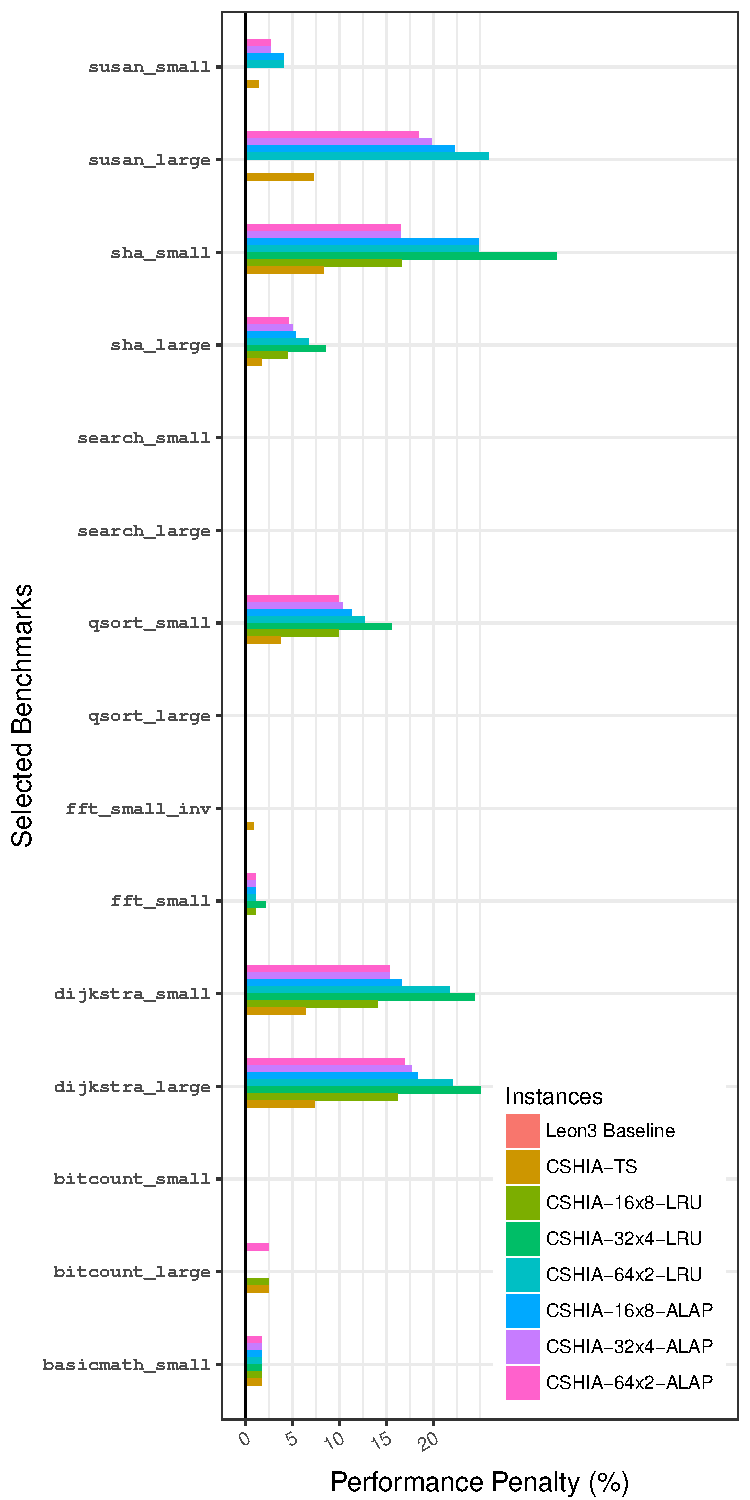
\includegraphics[scale=0.7]{benchmarks.pdf}
%	\caption{Execution time for benchmarks. For each benchmark, the running time was normalized by Leon's running time.}
%	\vspace*{-9pt} 
%	\label{fig:benchmarks}
%\end{figure}

\begin{table*}[t]
	\center
	\caption{Performance overhead in \% of the evaluated \cshia~instances in comparison of running times in \baseline.}
	\label{tab:results}
	\footnotesize
	\begin{tabular}{|l|c|c|}
%\		\noalign{\hrule height 1pt}
%\		\rowcolor{lightgray}
		\hline

	    Benchmarks				& \timestamp (\%)	& \cshiamt~instance(64x2-\lru)(\%)\\

		\hline
		\hline
		\texttt{qsort\_small}				& 	3.77	&	9.90\\
		\texttt{qsort\_large}				& 	0.05	&	0.05\\
		\texttt{bitcount\_small}			& 	0.00	&	0.00\\
		\texttt{bitcount\_large}			& 	2.43	&	0.00\\
		\texttt{sha\_small}					& 	8.31	&	16.55\\
		\texttt{sha\_large}					& 	1.78	&	4.75\\
		\texttt{search\_small}				& 	0.10	&	0.00\\
		\texttt{search\_large}				& 	0.00	&	0.01\\
		\texttt{fft\_small}					& 	0.00	&	1.07\\
		\texttt{fft\_small\_inv}			& 	0.92	&	0.00\\
		\texttt{dijkstra\_small}			& 	6.40	&	14.09\\
		\texttt{dijkstra\_large}			& 	7.35	&	16.90\\
		\texttt{basicmath\_small}			& 	1.73	&	1.73\\
		\texttt{susan\_small}				& 	1.37	&	2.73\\
		\texttt{susan\_large}				& 	7.23	&	18.72\\
		\hline
		\textit{\textbf{Average}}			&	\textbf{2.76}	&	\textbf{5.77}\\

		\hline
	\end{tabular}
%\vspace*{-12pt}
\end{table*}

Table \ref{tab:results} shows our results. The first conclusion is that \timestamp~performs better than the instance using the \mt. \timestamp~worst performance penalty is 8.30 \% for \texttt{sha\_small} and has an average performance penalty of just 2.76 \%. Because \cshia~could not entirely cover \texttt{sha\_large}, its performance penalty ended up being smaller than its counterpart. The \texttt{bitcount} and \texttt{fft} benchmarks had inconsistent results in some cases, when comparing all instances together. Delving into reasons for that, we found out that they are dependent of random number generation and this was affected by the intervention of \cshia~in the \amba~bus. Therefore, for those benchmarks, the performance difference between \cshia~instances should not be considered significant. Another observation regards to \texttt{qsort\_small} and \texttt{qsort\_large}. They presented similar behavior of the \texttt{sha}~benchmarks, despite \cshia~almost entirely covers the data segment of \texttt{qsort\_large}. 

Because verification of \ptags~of code memory blocks is equal in \timestamp~and \cshiamt, the only way to improve performance of \cshia~is reducing the number of accesses to \ptagmem~for data memory blocks. Thus, increasing the \ptag~cache size may lead \cshiamt~to obtain better performance than \timestamp. Obviously, these choices need to take into account other variables such as area and power, which we discuss next.

\section{Area and Power Estimates}
\label{subsec:Power-and-Area-Estimative}

Since we did not have access to standard tools from industry to synthesize \vhdl, we used the area and power proportionality relation \cite{Nemani1999:Area-Power} to compute our estimations. For that, we used well-known open tools like \cacti~5.3 \cite{HP:Cacti53} for cache memories estimative of power and area, and Ahmed \etal's work~\cite{Ahmed2009:Leon} that presents area and power for a synthesized \leon~processor on 65 nm LPLVT (Low Power Low Voltage Threshold) process using ST Microelectronics libraries.

Ahmed \etal~presented their \leon~design separating area, static and dynamic power for the core and its cache memory. We ignore their cache memory values since they differ from our implementation. Moreover, our primary goal is to estimate the area of logic elements. Thus, we will assume a proportional relation between their core area, 0.191 mm$^{2}$, and the number of \fpga~logic elements of the \baseline~implementation, which is 23,629 in the Altera's DE2-115 development kit. %tat static power (at 25\textordmasculine) 85.3 $\mu$W and dynamic power (at 100 MHz) was 5.75 mW. Although \cshia's~\fpga~implementation runs at 50 MHz, we can use Ahmed \etal~results to estimate \cshia's area overhead. As well as, for power, we can compute \leon's and \cshia's power using Intel's Early Power Estimators (\epe) \cite{Intel:EPE} for \fpgas~and deduce an estimative based on the ASIC power consumption of Ahmed \etal

Through this proportional relation between area and logic elements, our estimate for the \timestamp~and \cshiamt, without additional memories, is 0.246 mm$^{2}$ and 0.264 mm$^{2}$, respectively. As we said, area and power can be proportional, and thus we can use similar reasoning to estimate power. From Ahmed \etal's work, static and dynamic power (at 100 MHz) are 85.3 $\mu$W and 5.75 mW, respectively. Those numbers result in static power of 109.48 $\mu$W for \timestamp~and 117.41 $\mu$W for \cshiamt. In terms of dynamic power, we obtained 7.41 mW for \timestamp~and 7.94 mW for \cshiamt.

We used \cacti~to estimate how the timestamp memory and \ptagcache~affects the design. From Table \ref{tab:config}, the total timestamp memory size was 2 bytes $\times~2^{14}$ (or 32 KB). Even though \cacti~does do not offer an option for non-volatile estimative, a DRAM like estimation provides an insight of area and power. For the \ptagcache, we estimated 4-KB \ptagcache~with 64 lines and two sets, all estimations are summarized in Table \ref{tab:area-power}. 

\begin{table}[t]
	\center
	\caption{Area and power for \cshia~implementation~without considering instruction and data cache memories of the processor.}
	\label{tab:area-power}
	\footnotesize
	\begin{tabular}{|l|l|p{0.65in}|p{0.6in}|}
%\		\noalign{\hrule height 1pt}
%\		\rowcolor{lightgray}
		\hline
			\multirow{2}{*}{Instance} & \multirow{2}{*}{Area (mm$^{2}$)} & Static & Dynamic\\ 
			 & & Power (mW) & Power (mW)\\ 
		%\noalign{\hrule height 0.75pt}
		\hline
		\hline
			\baseline & & & \\
				\hspace{0.25in} Core & 0.191 & 85.3 $\times~10^{-3}$ & 5.75 \\
			\timestamp & & & \\
				\hspace{0.25in} Core & 0.246 & 109.48 $\times~10^{-3}$ & 7.41 \\
				\hspace{0.25in} Memory & 0.141 & 72.00 & 7.15  \\
				\hspace{0.25in} \textbf{Total} & 0.387 & 72.11 & 14.56  \\
			\cshiamt-64x2 & & & \\
				\hspace{0.25in} Core & 0.264 & 117.41 $\times~10^{-3}$ & 7.94 \\
				\hspace{0.25in} Cache & 0.274 & 6.90 & 100.98  \\
				\hspace{0.25in} \textbf{Total} & 0.538 & 7.02 & 108.92 \\
		\hline
	\end{tabular}
%\vspace*{-12pt}
\end{table}

Even if our estimates are not very accurate, they allow to analyze which solution would provide the best trade-off among area, power, and performance penalties. Thus, based on our numbers, the \timestamp~would be the best solution. Of course, that would only apply to this specific memory size we evaluated. In the security side, 16-bit timestamps will not provide the same security as our \cshiamt~instances with \ptags~of 64 bits. In addition, if the coverage of the data segment needs to be increased, the timestamp memory can reach prohibitive configurations for power and area. In such a situation, \cshiamt~would be capable of offering this higher coverage without impacting in on-chip power and area. Nonetheless, higher penalties in performance would happen. 
